\documentclass[../main.tex]{subfiles}
\begin{document}

\section{Notation \& Definitions}
In this section we introduce a mathematical description of the visualization pipeline where artist $A$ functions transform data of type $\Gamma(E)$ to an intermediate representation in prerendered display space of type $\Gamma(H)$:

\begin{equation}
    \label{eq:artist}
    A: \mathcal{O}(E) \rightarrow \mathcal{O}(H)
\end{equation}

\begin{itemize}
\item $A$ is the function that converts an instance of data $\Gamma(E)$ to an instance of a visual representation $\Gamma(H)$ 
\item $E$ is a locally trivial fiber bundle over $K$ representing data space.
\item $K$ is a triangulizable space encoding the connectivity of the points in $E$
\item $H$ is a fiber bundle over $S$ representing visual space
\item $S$ is a simplacial complex encoding the visualization
\end{itemize}

When $E$ is a trivial fiber bundle $E = F \times K$, it can be assumed that all fibers $F_{k}$ over $k \in K$ are equal. Fiber bundles are product spaces of toplological spaces, which are a set of points with a set of neighborhoods for each point\cite{FiberBundle2020, rowlandFiberBundle}.

\subsection{Fiber Bundles}
We provide a brief description of fiber bundles because we model data, visual transformations, and a prerendered visual graphic as fiber bundles. A fiber bundle is a structure $(E, B, \pi, F)$  consisting of topological total space $E$, base space $K$, fiber space $F$ and the map from total space to base space:

\begin{equation}
    \label{eq:fiber_bundle}
    \begin{tikzcd}
        F \arrow[r, hook] & E \arrow[r, "\pi"] & B
    \end{tikzcd}
\end{equation}

where there is a bijection from $F$ to every fiber $F_b$ over point $b \in B$ in $E$ and the function $\pi: E \rightarrow B$ is the map into the $B$ quotient space of $E$. By defintion of a fiber bundle, $\pi$ is always a mapping from total space to base space, independent of the points $p \in E$, and therefore we call this mapping $\pi$ for all the fiber bundles in the model. 

\subsubsection{Base space}
\begin{figure}[ht]
    \label{fig:base_space}
    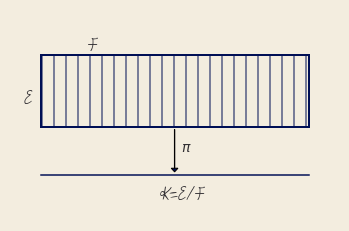
\includegraphics[width=0.4\linewidth]{figures/sections/math/k_qspace.png}
\end{figure}

$B$ is the quotient space of $E$, meaning it is the set of equivalence classes of elements $p$ in $E$ defined via the map $\pi: E \rightarrow B$ that sends each $p \in E$ to its equivalence class in $[p] \in B$ \cite{QuotientSpaceTopology2020,QuotientSpaceTopology2020}.

As shown in figure~\ref{fig:kquote}, the fibers $F$ divide $E$ into smaller spaces consisisting of $F$ and an open set neighborhood around $F$. This subdivision is projected down to the toplology $\mathcal{T}$

\begin{equation}
    \label{eq:base_space}
\mathcal{T}_b = \{U\subseteqq B: \{p \in E: [p] \in U\}\in \mathcal{T}_E\}
\end{equation}

where $[p] \in U$ is the point $b \in B$ with an open set surrounding it that has an open preimage in $E$ under the surjective map $\pi: p \rightarrow [p]$. 

\subsubsection{Fiber}
As shown in equation!\ref{eg:base_space}, every point $b \in B$ has a local open set neighborhood $U$ \cite{FiberBundle2020, rowlandFiberBundle}

\begin{equation}
    \label{eq:fiber_local_trivial}
    \begin{tikzcd}
        \pi^{-1}(U) \arrow[r, "\varphi"] \arrow[d, "\pi"'] & U \times F \arrow[ld, "\mathrm{proj}_U"] \\
        U                                                  &                                         
    \end{tikzcd}
\end{equation}
such that $\varphi: \pi^{-1}(U) \rightarrow U \times F$ is a homeomorphism where $\pi$ and $\mathrm{proj}_U$ both map to $U$ and the fiber over $k$ $F_b = \pi^{-1}({b \in B}) $ is homomorphic to the fiber $F$.

\subsubsection{Section}
The section $f$ is the mapping from base space to total space $f: B\rightarrow E$ 
\begin{equation}
    \label{eq:section}
    \begin{tikzcd}
        F \arrow[r, hook] & E \arrow[d, "\pi"']           \\
        & B \arrow[u, "f"', bend right]
    \end{tikzcd}
\end{equation}

such that $f$ is the right inverse of $\pi$
\begin{equation}
    \label{eq:section_domain}
    \pi(f(b)) = b \text{ for all } b \in B 
\end{equation}

In a locally trivial fiber bundle, $E = B \times F$ \cite{rowlandFiberBundle,FiberBundle2020}:
\begin{equation}
    \label{eq:section_return}
f(b) = (b, g(b))
\end{equation}

where the domain of $g(b)$ is $F_b$ and returns a point $p$ in $F_b$. The space of all possible sections $f$ of $E$ is $\Gamma(E)$. All sections $f \in \Gamma(E)$ have the same fibers $F$ and connectivity $B$. 

\subsubsection{Sheaf and Stalk}
As described in equation~\ref{eq:local_trivial}, there is a local space $U \subset B$ around every $b$. The inclusion map $\iota: U \rightarrow B$ can be pulled back such that $\iota^{*}E$ is the space of $E$ restricted over $U$. 
\begin{equation}
    \label{eq:sheaf}
    \begin{tikzcd}
        \iota^*E \arrow[d, "\pi"']           & E \arrow[d, "\pi"'] \arrow[l, "\iota^*"']         \\
        U \arrow[u, "\iota^*f"', bend right] & B \arrow[u, "f"', bend right] \arrow[l, "\iota"']
        \end{tikzcd}
\end{equation}

The localized section of fibers $\iota^*f: U \rightarrow \iota^*E$ is the sheaf $\mathcal{O}(E)$ with germ of $\xi^*f$. The neighborhood of points the sheaf lies over is the stalk $\mathcal{F}_b$ \cite{StalkSheaf2019,spanier1989algebraic}

\begin{equation}
    \label{eq:stalk}
    \iota^{-1}\mathcal{F}(\{b\}) = \varinjlim_{b\subseteq U}\mathcal{F}(U) =  \varinjlim_{b \in U} = \mathcal{F}_b 
\end{equation}

which through $\iota$ gets the data in $E$ at and near to $b$. Restricting the artist to the sheaf means the artist knows the data in $F$ and also has access to derivatives of the data. This property is useful for some visual transformations. 
%% gives all direvatives but we need the jet which is Add stuff about jets

\subsection{Data Model}
As proposed by Butler \cite{butlerVectorBundleClassesForm1992,butlerVisualizationModelBased1989}, we model data as a fiber bundle (E, K, $\pi$, F) with $\pi: E \rightarrow K$ where $K$ which can be thought of as a set of keys $k$. A section $\tau:K \rightarrow E$ is an instance of the data that lies in $E$ and is discussed in section~\ref{sec:data_fiber}. 

\subsubsection{Example}

\begin{figure}[ht]
    \label{fig:data_fiber_bundle}
    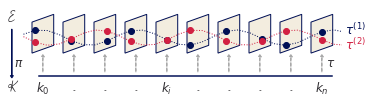
\includegraphics[width=.2\linewidth]{figures/sections/math/fiberbundle.png}
    \caption{write up some words here}
\end{figure}

As illustrated by figure~\ref{fig:fiberbundle}, the vertical lines $F$ are the range of possible temperature values embedded in the total space $E$. The base space $K$ of the fiber bundle is a line because the data points $r$ in $E$ are on a space that is  continous in one dimension. 

\subsubsection{Base Space}
The base space $K$ is a representation of the connectivity of the data, specifically whether the points in $E$ are discrete or sampled from a continous space. The same dataset can be expressed with different $K$. 

\subsubsection{Example}
\begin{figure}[ht]
    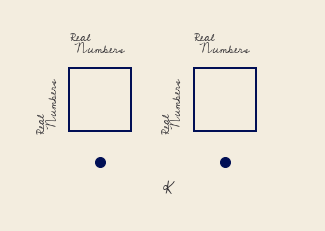
\includegraphics[width=0.2\linewidth]{figures/sections/math/temp_1k.png}
    %% add box around neighboring P and Map
    \label{fig:k_data}
\end{figure}

\begin{figure}[ht]
    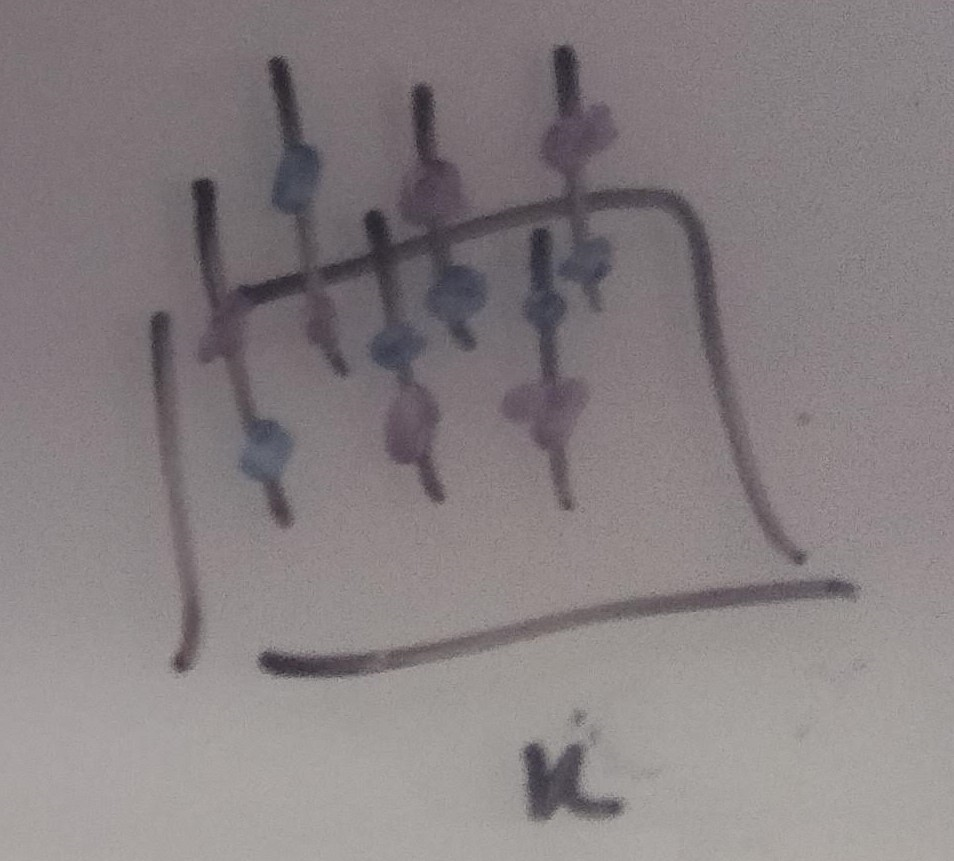
\includegraphics[width=0.2\linewidth]{figures/sections/math/temp_2k.png}
\end{figure}

in figure~\ref{fig:k_data}, temperature is the only one data field in $r$ but the $K$ base spaces are different. subfig[1] is a timeseries, so the temperature in $r$ at time $t$ is dependent on the temperature in $r_{t-1}$ and the temperature in $r_{t+1}$ is dependent on  $r_t$; this connectivity is expressed as a one dimensional $K$ where $K$ is the number line. In the case of the map, every temperature in $r$ is dependent on its nearest neighbors on the plane, and one way to express this is by encoding $K$ as a plane. $K$ does not know the time or latitude or longitude of the point as those are metadata variables describing the $k$ rather than the value of $k$. The mapping $\tau: K \rightarrow E$ provides the binding between the key $k \in K$ and the value $r$ in $E$ \cite{munznerChDataAbstraction}.

\subsubsection{Fiber and Sections}
\label{sec:data_fiber}
We use Spivak's formalization of data base schemas as the basis of our fiber space $F$ \cite{spivakSIMPLICIALDATABASES}. He defines the type specification 
\begin{equation}
\pi: U \rightarrow DT
\end{equation}

where $DT$ is the set of data types (as identified by their names) and $U$ is the disjoint set of all possible objects $x$ of all types in $DT$. This means that for each type $T\in DT$, the preimage $\pi^{-1}(T)\subset U $ is the domain of $T$, and $x \in \pi^{1}(T)\subset U$ is an object of type $T$. Spivak then defines a schema $(C, \sigma)$ of type $\pi$, where $\pi$ is the universe of all types, such that 
\begin{equation}
\sigma: C \rightarrow DT
\end{equation}
where $C$ is the finite set of names of columuns, which we generalize to data fields in $E$. The set of all values restricted to the datatypes in $DT$ is $U_{\sigma}$

\begin{equation}
    \begin{tikzcd}
        U_{\sigma} \arrow[d, "\pi_{\sigma}"'] \arrow[r] & U \arrow[d, "\pi"] \\
        C \arrow[r, "\sigma"]                           & DT                
    \end{tikzcd}
\end{equation}
The pullback $U_{\sigma} \coloneqq \sigma^{-1}(U)$ restricts $U$ to the datatypes of the fields in $C$ such that $U_{\sigma}$ is the fiber product $U \times_{DT} C$, and the pullback $\pi_{\sigma}:U_{\sigma} \rightarrow C$ specifies the domain bundle $U_{\sigma}$ over $C$ induced by $\sigma$. The fiber $F$ is the cartesian product of all sets in the disjoint union $U_{\sigma}$. 

For each field $c \in C$, the record function $r: C \rightarrow U_{\sigma}$ returns an object of type $\sigma(c) \in DT$. The set of all records $\Gamma(\sigma)$ is the set of all sections on $U_\sigma$. Spivak defines the $\tau$ mapping from an index of databases $K$ to records $\Gamma(\sigma)$ as $\tau: K \rightarrow \Gamma(\sigma)$. This is equivalent to $\tau: k \rightarrow E$ since $F = \Gamma(\sigma)$ and $F$ is the embedding in $E$ on which the records $r$ lie.
 
\subsubsection{Example}
\begin{figure}[ht]
    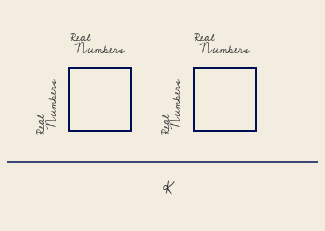
\includegraphics[width=0.2\linewidth]{figures/sections/math/temp_2f.png}
    \label{fig:}
\end{figure}
\begin{figure}[ht]
    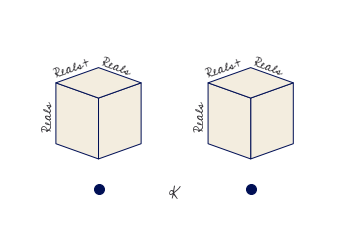
\includegraphics[width=0.2\linewidth]{figures/sections/math/temp_3f.png}
\end{figure}


%% pull out measurement
The fiber in figure~\ref{fig:temp} is the space of possible temperature values in degrees celsius, such that $F=[temp_{min}, temp_{max}]$ and is named \textrm{Temp}. In figure~\ref{fig:temp_time} \textrm{time} is encoded as a second dimension. This means that the set of possible values $F$ with $C=\{\textrm{Temp}, \textrm{Time}\}$:

\begin{equation}
F = [temp_{min}, temp_{max}] \times [time_{min}, time_{max}]
\end{equation}

and the function $\tau$ that retrieves records from $F$ is

\begin{align}
\tau(k) =(k, (r: \textrm{Temp}\rightarrow &temp, r: \textrm{Time}\rightarrow time))\\
&temp \in [temp_{min}, temp_{max}], time \in [time_{min}, time_{max}])
\end{align}

Since $\tau(k)=(k, r)$, $temp$ is bound to a named data field and $sigma$ binds $temp$ to a temperature data type. 

\subsection{Prerender Space}
\label{sec:display}
We model the prerender space on which lives on ideal version of the visulaization as a fiber bundle (H, S, $\pi$, D). $H$ is the predisplay space, with a fiber $D$ dependent on the target physical display and a base space of $S$. 

\subsubsection{Base space}
$K$ can be considered a subspace of the screen base space $S$ such that $\xi: S \rightarrow K$ is a deformation retraction \cite{RetractionTopology2020}
\begin{equation}
    \begin{tikzcd}
        E \arrow[d, "\pi"'] & H \arrow[d, "\pi"'] \\
        K                   & S \arrow[l, "\xi"']
        \end{tikzcd}
\end{equation}

that goes from a region $s \in S_{k}$ to its associated point $k$, such that when $\xi(s) = k$, $\xi^*\tau(s) = \tau(k)$. 

\subsubsection{Fiber and Section}
A section $\rho: S \rightarrow H$ is a mapping from a region $s$ on a mathematical encoding of the image to a region $xy$ on the screen that the renderer then maps to visual space as defined in D. For a physical screen display, the predisplay space is a trivial fiber bundle $H=\mathbb{R}^{7}\times S$ such that $\rho$ is
\begin{equation}
    \rho(s)  = \{x, y, z, r, g, b, a\}
    \label{eq:rho}
\end{equation}

To draw an image, a region, $H$ is inverse mapped into a region $s \in S$ where
\begin{equation}
s = \rho^{-1}_{\tiny{XY}}(xy)
\end{equation}
such that the rest of the fields in $\mathbb{R}^{7}$ are then integrated over $s$ to yield the remaining fields:
\begin{align}
    r &= \iint\limits_s \rho_{\tiny{R}}(s)ds^{2}\\
    g &= \iint\limits_s \rho_{\tiny{G}}(s)ds^{2}\\
    b &= \iint\limits_s \rho_{\tiny{B}}(s)ds^{2}
\end{align}

Here we assume a single opaque 2D image such that the $z$ and $alpha$ fields can be omitted. 

\subsubsection{{Example}}
\begin{figure}[h]
    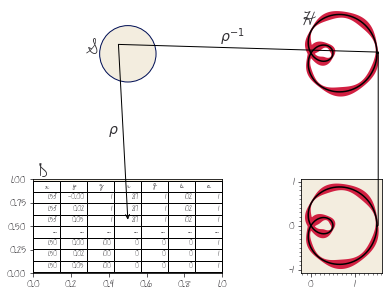
\includegraphics[width=.4\linewidth]{figures/sections/math/render.png}
    \caption{}
    \label{fig:render}
\end{figure}

As illustrated in figure~\ref{fig:render}, words.

\subsection{Artist}

In this section we will define the artist as a mapping from a sheaf $\mathcal{O}(E)$  to $\mathcal{O}(H)$. 
\begin{equation}
    A: \mathcal{O}(E) \rightarrow \mathcal{O}(H)
\end{equation}

The artist decomposes to mapping data to visual $\nu:E\rightarrow V$, then  compositing $V$ pulled back along $\xi$ to $\xi^*V$ to a visual mark in prerender space $Q:\xi^*V\rightarrow H$. 

\begin{equation}
    \label{eq:artist}
\begin{tikzcd}
    E \arrow[r, "\nu"] \arrow[rd, "\pi"'] & V \arrow[d, "\pi"] & \xi^*V \arrow[r, "Q"] \arrow[d, "\xi^*\pi"'] & H \arrow[ld, "\pi"] \\
                                          & K                  & S \arrow[l, "\xi"']                          &                    
\end{tikzcd}
\end{equation}

The visual fiber bundle ($V$, $K$, $\pi$, $P$) has section $\mu: V \rightarrow K$ that resolves to a visual variable \cite{bertinIIPropertiesGraphic2011,munznerMarksChannels} in fiber $P$. The visual transformer $\nu$ is a set of functions each targeting a different $\mu$
\begin{equation}
    \label{eq:nu_expanded}
    \nu:\{\nu_{0}, \ldots, \nu_{n}\} \rightarrow \{\mu_{0}, \ldots, \mu_{n}\}
\end{equation}

where $\mu_{i}$ are the visual parameters in the assembly function $Q(\mu_{0}, \ldots, \mu_{n})(s) = \rho(s)$. 


\subsubsection {Example: Matplotlib Visual Fiber}
For example, for Matplotlib \cite{hunterMatplotlib2DGraphics2007}, some of the possible types in $P$ are:
\begin{table}[ht]
    \label{tab:mpl_visual_variable_fiber}
    \renewcommand{\arraystretch}{2}
    \begin{tabulary}{\textwidth}{|l|L|l|}\hline
     $\bm{\nu_{i}}$                      & $\bm{\mu_{i}}$                                                            & $\bm{codomain(\nu_{i})}$  \\ \hline                                              
    position                    & x, y, z, theta, r                                                          & $\mathbb{R}$   \\ \hline
    size                        & linewidth, markersize                                            & $\mathbb{R}^{+}$   \\ \hline
    shape                       & markerstyle                                                      & $\{f_{0}, \ldots, f_{n}\}$ \\ \hline
    color                       & color, colors, linecolor, facecolor, markerfacecolor, edgecolor  & $\mathbb{R}^4$ \\ \hline
    \multirow{2}{*}{texture}    & hatch                                                            & $\mathbb{N}^{10}$\\\cline{2-3}
                                & linestyle                                                        & $(\mathbb{N}, \mathbb{N}^{n})$ \\ \hline              
    \end{tabulary}
\end{table}

\subsubsection{Visual Channels}

A monoid is a set with a closed operation 



The function $\nu: E \rightarrow V$ is a mapping from the data bundle to the visual bundle 
\begin{equation}
    \label{eq:nu_categorical}
\begin{tikzcd}
    E_i \arrow[r] \arrow[r, "\nu_i"] \arrow[d, "f"'] & V_i \arrow[d, "f"] \\
    E_i \arrow[r, "\nu_i"]                           & V_i               
\end{tikzcd}
\end{equation}

such that a visual section $\mu: K \rightarrow V$  is equivalent to the visual transformation of the data $\mu(k) = \nu\circ\tau(k)$



The Stevens measurement scales\cite{stevensTheoryScalesMeasurement1946,leaFormalizationMeasurementScale} are examples of some of the group actions th


+2 on data side means +2 on visual side 


.2 = E1 - lambda e -> .2 V1 = .2
+.2                              +.2
.4 = E2 - lambda e -> .2 V2 = .2

.2 = E1  - lambda e-> .2 V1 = .2

                        V2 = .2

1 = E1 - lambda e->e/5 = .25

+ 1                      +.25 

2 = E2 - lambda e->e/5 = .5


preserve unique mapping? does $\nu$ need to be invertable? 

shifts in either space need to be mirrored in the other space, this is not valid  here's why:
$\lambda e: .2$ 
\begin{equation}
    \label{eq:nu_equation_bad}
    \begin{tikzcd}
        E_1 \arrow[r] \arrow[r, "\lambda:e\mapsto.5"] \arrow[d, "e+2"'] & V_1 \arrow[d, "h+2"] \\
        E_2 \arrow[r, "\lambda"]                                        & V_2                 
    \end{tikzcd}
\end{equation}

{x,y} = {1,2}
{y,x} = {2,1}
{y,x} = {1,2}



\subsubsection{Constructing Marks}
The visual fiber bundle $V$ gets pulled back over $S$ via $\xi$ such that 
\begin{equation}
    \begin{tikzcd}
        \xi^*V \arrow[r, "Q"] \arrow[rd, "\xi^*\pi"'] & H \arrow[d, "\pi"] \\
                                                      & S                 
    \end{tikzcd}
\end{equation}
the function $Q:\xi^*V\rightarrow H$ composites points in $V$ into $\mathbb{R^7}$ tuples. The section $\mu$ is pulled over $s$ 

\begin{equation}
    \begin{tikzcd}
        \xi^*V \arrow[r, "Q"] & H                                           \\
                              & S \arrow[lu, "\xi^*\mu"] \arrow[u, "\rho"']
    \end{tikzcd}
\end{equation}

such that the composition $Q$ of $\mu$ is equivalent to the render $\rho(s) = Q\circ\mu(s)$. 
(In practice $\mu \approxeq \xi^*\mu$)
$Q$ is the constructor for the mark, 
one $Q$ per artist, A = sum of artists
$Q$ as there's default line, point, etc that's stretched and tweaked and whatever else by the $\mu$
visual variable + structure preserving, Q must have map that commutes such that a change in $\mu$ carries over somehow to $\rho$, functorial in its arguments - commutative diagram - into rho

\end{document}